El filtro rotar consiste en realizar una rotación de la imagen original.

Rotar es el menos capacitado para paralelización. Esta dificultad proviene de la imposibilidad de leer bytes y procesarlos simultaneamente debido a que el valor de cada pixel en la imagen destino se obtiene calculando, según su posición, qué pixel corresponde de la imagen fuente, lo que implica traer uno a uno los pixeles de la imagen fuente para colocarlos en en lugar indicado en la imágen destino.

Analizando el algoritmo, llegamos a la conclusión de que la mejor manera de explotar la simultaneidad que nos brinda las instrucciones SIMD, es utilizarlas para calcular las posiciones de dónde sacar el pixel para colorcarlo en la imagen destino. 

Inicialmente este proceso fue realizado utilizando single precision floats para poder aprovechar SIMD al máximo y realizar cálculos para conseguir las posiciones de donde sacar los pixeles a la vez. Este intento se vió frustrado al correr el filtro y compararlo contra las imágenes provistas por la cátedra. Si bien la imagen coincidía visualmente, se encontraron errores en 27 pixeles. Un análisis de estos pixeles pusieron en evidencia un problema de precisión, el cual se intentó arreglar utilizando la instrucción roundps sin conseguir mejores resultados. Se solucióno el problema realizando los cálculos usando double precision floats con SIMD para luego convertirlos a floats y finalmente convertirlos a enteros para poder funcionar como posición.

\subsubsection{Descripción del ciclo}
El filtro se divide en cinco etapas:
\begin{enumerate}
\item \textbf{Pre-ciclo principal e inicio:} Se crean ciertos registros que serán de utilidad en el ciclo.
\item \textbf{Ciclo para obtención de posiciones:} Se obtiene mediante un ciclo los valores de x e y para las siguientes cuatro posiciones.
\item \textbf{Cálculo de u y v:} Cálculo de los valores u y v correspondientes a x e y en la imagen fuente.
\item \textbf{Ciclo de almacenamiento de los valores correspondientes a las posiciones procesadas:} Se buscan los valos de los pixeles en la imagen fuente que se escribirán en la imagen destino.
\item \textbf{Escritura de los pixeles en la imagen destino y fin del ciclo principal:}
\end{enumerate}

\subsubsection{Pre-ciclo principal}
Para optimizar la implementación, se realiza el cálculo de cx, cy y $\sqrt[2]{2}/2$ al inicio del programa. Estos valores se almacenan en registros como doubles empaquetados utilizando \texttt{SHUFPS} para tener cáda valor en double words y luego convertirlos a doubles con \texttt{CVTDQ2PD}.

También se ponen en 0 los registros \reg{11} y \reg{15} que servirán para establecer en que posición x e y respectivamente se encuentra en la imagen.

El ciclo principal comienza poniendo en 0 mediante la instrucción \texttt{POR} el registro \xmm{7} el cuál se encargará de acumular los pixeles hasta llenarse sus 16 bytes.

\subsubsection{Ciclo para obtención de posiciones}
Este ciclo interno se encarga de poner en dos registros temporales los valores de las posiciones x e y de cuatro pixeles sucesivos. Una vez realizado esto, para poder trabajar con los cuatro pixeles utilizando doubles, se mueve el contenido de estos registros a registros \texttt{XMM} dónde se los convierte, utilizando \texttt{CVTDQ2PD} y se los almacena en cuatro registros \texttt{XMM}, dos con los dos doubles más bajos y altos de las coordenadas x y dos con los dos doubles más bajos y altos de las coordenadas y.

\begin{center}
    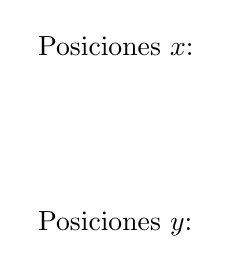
\begin{tikzpicture}[scale=0.75]
        \draw (0, 5) node[anchor=west]{Posiciones $x$:};
        
        \registroCuatro{}{0}{3}{0}{1}{2}{3}

        \draw (0, 2) node[anchor=west]{Posiciones $y$:};

        \registroCuatro{}{0}{0}{0}{0}{0}{0}
    \end{tikzpicture}
\end{center}
Ejemplo del estado de los registros \texttt{XMM} asignados para x e y en la primera iteración del ciclo principal

\subsubsection{Cálculo de u y v}
Se opera sobre los doubles utilizando instrucciones SIMD, obteniedo los valores u y v, es decir, los valores x e y respectivamente de dónde conseguir el pixel a poner en la imágen fuente.

Haciendo un análisis de las ecuaciones, decidimos realizar los cálculos de u y v de la siguiente manera:
\begin{itemize}
\item Dividir y calcular u como u1 y u2: u1 = cx + ($\sqrt[2]{2}/2$)*(x-cx) y u2 = -($\sqrt[2]{2}/2$)*(y-cy)
\item Dividir y calcular v como v1 y v2: v1 = cy + ($\sqrt[2]{2}/2$)*(x-cx) y v2 = +($\sqrt[2]{2}/2$)*(y-cy)
\end{itemize}

De esta manera se puede calcular con instrucciones SIMD, utilizando \texttt{SUBPD}, (x-cx), multiplicandolo después con \texttt{MULPD} por ($\sqrt[2]{2}/2$) y utilizando luego este resultado para formar v1 y u1 con la suma de cy y cx respectivamente. Por último calcular u2 y v2, ($\sqrt[2]{2}/2$)*(y-cy), de manera similar, restándolo a u1 y sumándolo a v1.

Al finalizar el cálculo se convierten de doubles a floats utilizando \texttt{CVTPD2PS}, de floats a enteros con \texttt{CVTTPS2DQ} y se shiftean hacia la izquierda los registros con las partes altas de x y de y (ahora u y v), mediante \texttt{PSLLQD}, para luego agregarles en la parte baja los valores de las partes bajas calculados utilizando la instrucción \texttt{POR}, dejando 4 double words packed con u's y 4 double words packed con v's.

\subsubsection{Ciclo de almacenamiento de los valores correspondientes a las posiciones procesadas}
Antes de empezar este ciclo, se pone el registro \rbp en 0 mediante un \texttt{XOR} ya que servirá como acumulador temporal del ciclo.

Se pasa a un pequeño ciclo el cuál mediante \texttt{MOVD} y \texttt{PSLLDQ} (que realiza un shift a la izquierda) saca de los registros las double words calculadas en el paso anterior con las u's y v's y checkea de a una las restricciones del cálculo para u y v, para luego colocar en el caso de que las cumplan, en el acumulador del ciclo, el valor del pixel que tenga en la posición en la imagen fuente (el cuál es leido desde esta) y si no, un 0.

Terminado el ciclo de almacenamiento, se agregan los valores de estos 4 bytes al acumulador principal creado al comienzo del ciclo, utilizando \texttt{PSLLDQ} para shiftearlo a la izquierda 4 bytes y agregando los valores mediante un por y se vuelve a ciclar realizando el mismo proceso hasta llenar el acumulador con los valores correspondientes de los 16 bytes o 16 pixeles contiguos.

\subsubsection{Escritura de los pixeles en la imagen destino y fin del ciclo principal}

En el final de cada iteración del ciclo princiapl, se checkea la posición de la imagen en la que se está (por si ya se ha terminado de recorrerla o se es necesario correr para atrás para agarrar 16 pixeles exactos) y si se ha llenado el acumulador. Si el acumulador se llena (habiendo pasado 4 ciclos) se escriben los 16 bytes a la imagen destino. Este mecanismo en el cuál se van almacenando los pixeles tiene como sentido economizar la escritura de datos.

\subsubsection{Comparación con la implementación C}
Cómo el algoritmo no es muy paralelizable, ambas implementaciones comparten varias características pero difieren en algunos casos, a continuación se detalla.

Operaciones realizadas en la implementación en C para 16 bytes:
\begin{itemize}
\item Se realizan 2x16 accesos a memoria, 16 para la lectura de un pixel determinado en la imágen fuente y otros 16 para la escritura en la imágen destino.
\item Se realiza el cálculo relacionado a u y v de manera secuencial.
\item Se realiza el checkeo de las restricciones para u y v de manera secuencial.
\end{itemize}

Operaciones realizadas en la implementación en ASM para 16 bytes:
\begin{itemize}
\item Se realizan 16 accesos a memoria para la lectura de un pixel determinado en la imágen fuente y 1 acceso utilizando movqdu para la escritura en la imágen destino.
\item Se realiza el cálculo relacionado a u y v utilizando instrucciones SIMD pudiendo realizar los cálculos con 2 datos simultáneos realizando en cáda ciclo 4 cálculos de u y v y en cada ciclo principal el cálculo de los 16 bytes.
\item Se realiza el checkeo de las restricciones para u y v de manera secuencial.
\end{itemize}

\subsubsection{Rendimiento}
Observamos las siguientes cantidades de ciclos y ticks de reloj al realizar 100 iteraciones de ambas implementaciones con una imagen cuadrada de lado 512.
\begin{center}
    \begin{tabular}{|l|l|l|l|}
        \hline
        Medición & Implementación C & Implementación assembler & Relación \\
        \hline
        Ticks    & 1766855008      & 727560304               & $41.17\%$ \\
        Ciclos   & 17668550       & 7275603                & $41.17\%$ \\
        \hline
    \end{tabular}
\end{center}

Es notable la diferencia en velocidad con los otros filtros. Este resultado pone en evidencia que al poder paralelizarse en menor manera que otros filtros, la velocidad y los ciclos aumentan considerablemente.

Cabe destacar que la diferencia de velocidad obtenida en comparación con la implementación en C no sólo proviene de el uso de instrucciones SIMD para el cálculo con doubles o el acceso a memoria usando movqdu, si no que también influyen el uso contínuo de registros en vez de accesos memoría para almacenar datos (algo que C hace) y la posibilidad que otorga el lenguaje ensamblador de ordenar el código para poder optimizar al máximo los algoritmos.